Cal mencionar que la llista de programari utilitzat per al projecte es
detalla en la SBOM. En aquest apartat ens centrarem només en el flux de
treball per programar les plaques FPGA.

\subsubsection{ Xilinx Vivado i Vitis IDE }
{ 
    Vivado és un programari propietari de Xilinx emprat per la programació de
    la fàbrica lògica de les seves FPGA i SoCs.

    \begin{figure}[ht]
        \centering
        \captionsetup{justification=centering,margin=1.5cm}
        \includegraphics[width=10cm, height=6cm]{example-image-a}
        \caption{ Vivado }
    \end{figure}

    Vitis IDE, per la seva altra banda, és un entorn de desenvolupament
    basat en Eclipse IDE amb la qual es pot realitzar de manera integrada
    la programació, la compilació i el desplegament d'aplicacions, amb les
    seves respectives plataformes (bare-metal, freertos o linux).

    en un primer lloc és necessari instal·lar el programari visitant el
    centre de descàrregues de Xilinx\footnotemark.

    \footnotetext{ \url{https://www.xilinx.com/support/download.html} }

    \begin{figure}[ht]
        \centering
        \captionsetup{justification=centering,margin=1.5cm}
        \includegraphics[width=10cm, height=6cm]{example-image-a}
        \caption{ Vitis IDE }
    \end{figure}
}

\subsubsection{ Vitis Model Composer }
{ 
    Vitis\texttrademark Model Composer és una extensió de
    Matlab\textsuperscript{\textregistered} que proporciona un blokset amb
    el qual descriure i implementar la lògica programable. Anteriorment a
    2019, l'eina es comercialitzava baix el nom de \emph{System Generator},
    per la qual cosa encara apareix aquest nom en gaire documentació.

    Per utilitzar aquesta eina, haurem de comprobar que la versió de
    Matlab\textsuperscript{\textregistered} enllaçada amb el programa és la
    desitjada. Per defecte, Vitis escull la versió compatible més recent en
    el moment de la instal·lació. Quan iniciem el programa seleccionant la
    seva icona en l'escriptori o en el menú d'aplicacions, s'importen
    variables necessàries per habilitar l'entorn dins de Simulink. Per
    començar a desenvolupar lògica programable, basta amb seleccionar
    l'icona de Simulink i crear o obrir un model de Simulink (\emph{.xls}).

    \begin{figure}[!htb]
        \centering
        \captionsetup{justification=centering,margin=1.5cm}
        \includegraphics[width=10cm, height=6cm]{example-image-a}
        \caption{ Simulink amb el blockset de Vitis Model Composer }
    \end{figure}

    El blockset de Vitis Model Composer exten la llibreria de Simulink.
    S'ha de tenir en compte que els blocs nadius de Simulink no es
    sintetizen en hardware, sino que ens serveixen per dissenyar les
    simulacions i visualitzar els resultats. Per aquesta raó, existeixen
    uns blocs específics que actuen com entrada i sortida del hardware: són
    els blocs \emph{Gateway In} i \emph{Gateway Out}. Tots el blocs
    connectats a la sortida de \emph{Gateway In} i a l'entrada de
    \emph{Gateway Out} hauran de pertànyer al blockset de Model Composer,
    ja que es tradueixen directament en lògica progamable.

    \begin{figure}[!htb]
        \centering
        \captionsetup{justification=centering,margin=1.5cm}
        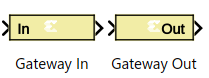
\includegraphics[width=5cm]
            { img/model_composer/gateways.png }
        \caption{ \emph{Gateway In} i \emph{Gateway Out} }
    \end{figure}

    Abans de començar a enllaçar blocs, s'ha d'afegir i configurar el bloc
    de \emph{System Generator}. És el bloc maestre del sistema i en
    seleccionar-ho podem, entre altres, modificar la freqüència de clock
    del sistema, \todo*{ Acabar explicació system generator }

    \begin{figure}[!htb]
        \centering
        \captionsetup{justification=centering,margin=1.5cm}
        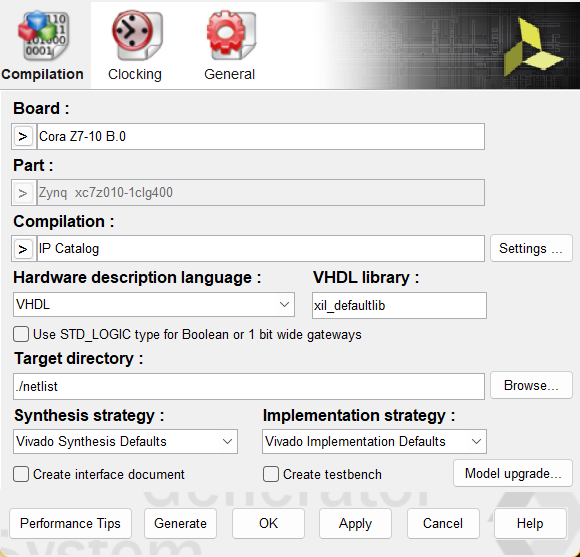
\includegraphics[width=7cm]
            { img/model_composer/sysgen_window.png }
        \caption{ Finestra de configuració de \emph{System Generator} }
    \end{figure}
}

\subsubsection{ Desenvolupament en C++ }
{ 
    Visual Studio Code és un editor de text versàtil desenvolupat per
    Microsoft per Windows, Linux, macOs i web. La versatilitat de l'editor
    prové de la posibilitat d'instalar extensions des de la botiga
    d'aplicacions \emph{VS Marketplace} i de configurar tasques per
    automatitzar processos com pot ser la compilació i el desplegament de
    progamari en plaques o en servidors externs. De fet, aquesta memòria
    s'ha realitzat fent ús d'aquest editor, mitjançant la seva corresponent
    extensió habilitadores \emph{LaTex Workshop} i una instal·lació de
    \LaTeX $\ $ per Windows, MikTex.

    \begin{figure}[!htb]
        \centering
        \captionsetup{justification=centering,margin=1.5cm}
        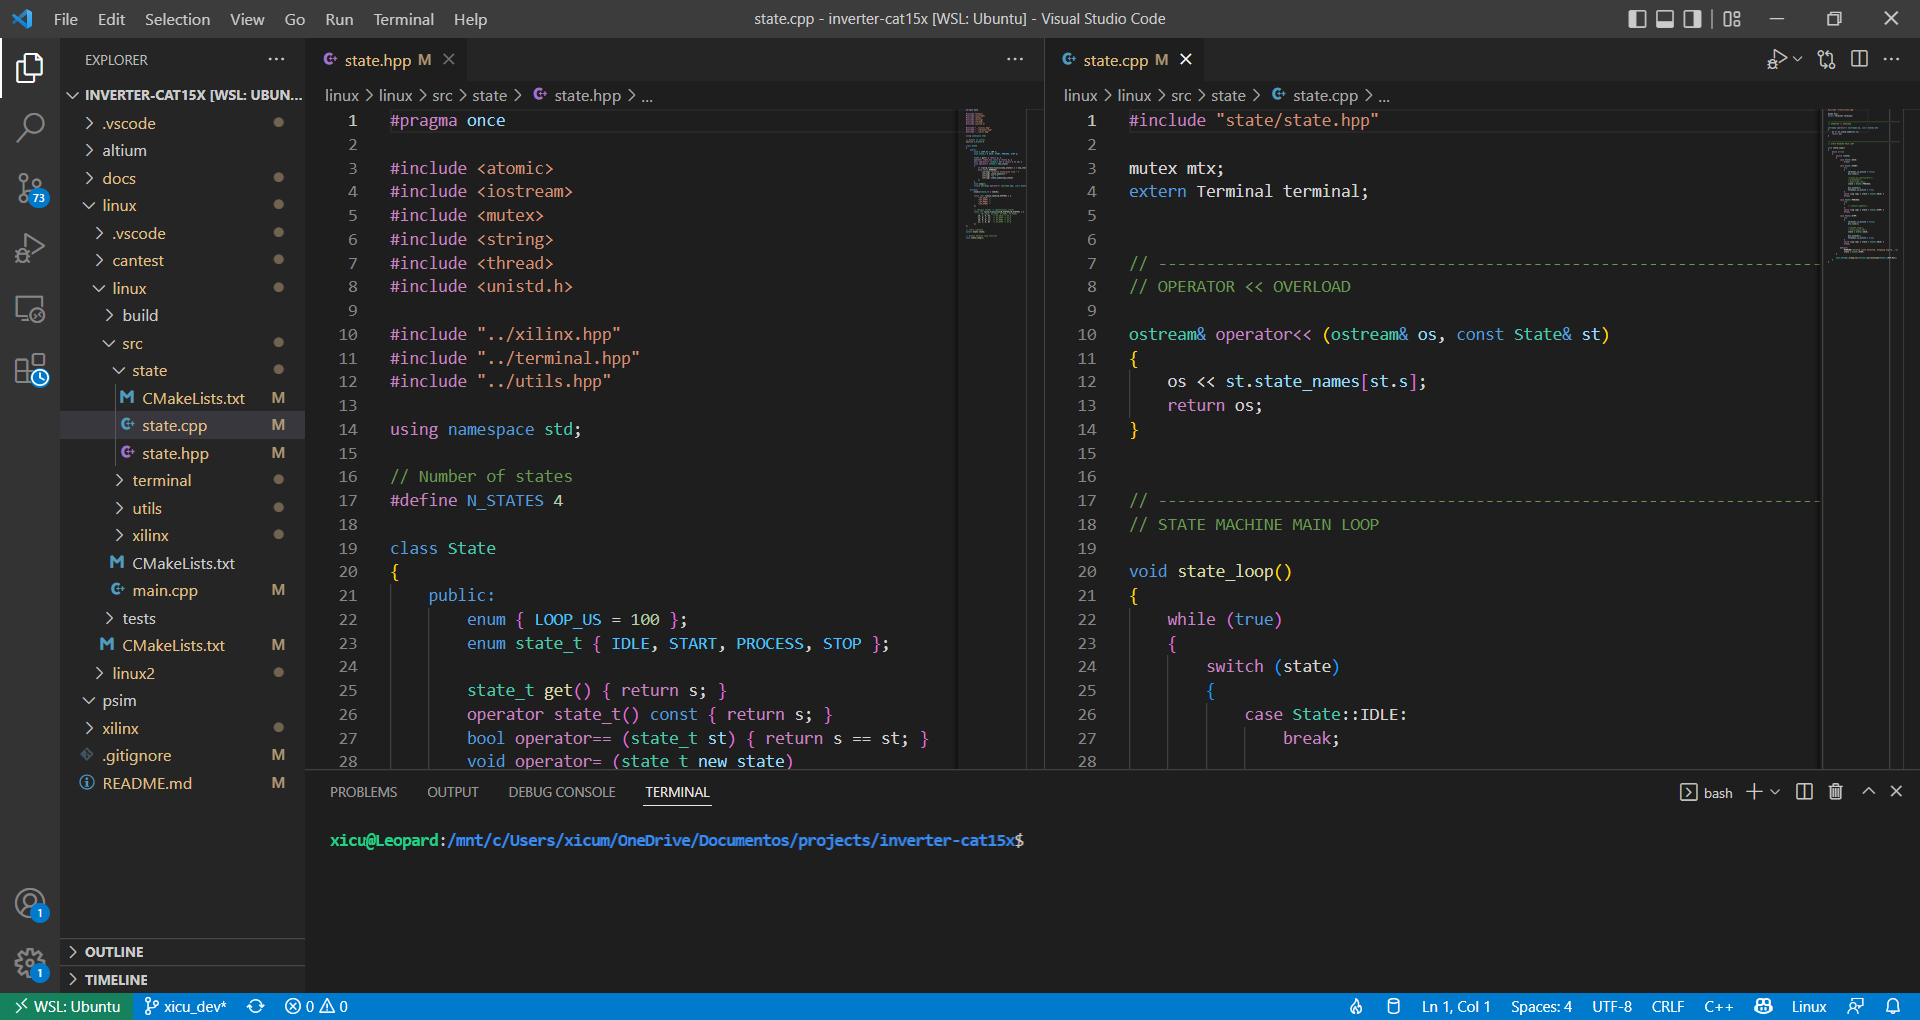
\includegraphics[width=15cm]
            { img/4_implementacio/VSCode.png }
        \caption{ Captura de pantalla de l'entorn Visual Studio Code }
    \end{figure}
}